\section{Systematics and expected sensitivity}
(outline by David)

\subsection{Test Statistic Definition}
The test statistic used in this analysis is the chi-square (\(\chi^2\)) statistic, calculated for comparing observed data with expected data, taking into account both statistical and systematic uncertainties. Mathematically, the chi-square statistic is defined as:

$$
\chi^2 = (\mathbf{n} - \boldsymbol{\mu})^T C^{-1} (\mathbf{n} - \boldsymbol{\mu})
$$

where \(\mathbf{n}\) is the vector of observed data, \(\boldsymbol{\mu}\) is the vector of expected data, and \(C^{-1}\) is the inverse of the total covariance matrix, \(\mathbf{C}\). 

The total covariance matrix is the sum of the systematic covariance matrix, \(C_{\text{sys}}\), and the statistical covariance matrix, \(C_{\text{CNP}}\):

\[
C = C_{\text{sys}} + C_{\text{CNP}}
\]

The systematic covariance matrix (\(C_{\text{sys}}\)) accounts for the systematic uncertainties in the experiment, while the statistical covariance matrix (\(C_{\text{CNP}}\)) accounts for the statistical fluctuations in the observed data.

The statistical covariance matrix \(C_{\text{CNP}}\) is a linear combination of the Neyman and Pearson chi-square constructions that has been shown to minimize the bias of the chi-square estimator when the data is Poisson distributed\todo{cite}. The CNP covariance matrix, \(C_{\text{CNP}}\), is defined element-wise for diagonal elements as:

\[
C_{\text{CNP}, ii} = \begin{cases} 
\frac{3 \mu_i n_i}{\mu_i + 2 n_i} & \text{if } n_i > 0 \\
\frac{\mu_i}{2} & \text{if } n_i = 0
\end{cases}
\]

where \(\mu_i\) and \(n_i\) are the expectation and observation in the \(i\)th bin, respectively. In cases where \(n_i = 0\), setting \(C_{\text{CNP}, ii} = \frac{\mu_i}{2}\) recovers the Poisson chi-square\todo{cite}. We ignore bins where the expectation value $\mu_i$ is zero. 

The systematic part of the covariance matrix, $C_\text{sys}$, is the sum of the covariance matrices from each source of systematic uncertainties that are described in the following sections. 

\subsection{Systematics: unchanged}

The treatment of systematic uncertainties in this updated analysis is largely the same as that of the runs 1-3 analysis. The reweighting treatment is employed for the flux, generator, and reinteraction systematics, and the same set of variations are employed to propagate detector uncertainties. The only significant changes are the inclusion of the off-diagonal elements of the covariance matrix for detector response related uncertainties, and the treatment of the EXT statistical uncertainty, both of which are described below.

\subsection{Systematics: What's new}

\subsubsection{GENIE FSI Bug-fix}
During validation of the MC samples from runs 4 and 5, it was discovered that the reweighted universes used to propagate systematic uncertainties related to cross section physics were not consistent\footnote{See docdb \#40416, \#40783, and \#41188 for more information on this subject.}. The cause was determined to be inconsistent versions of the code used to propagate FSI related uncertainties, with the ntuples produced for runs 1-3 being generated with the pre-FSI bug-fix version of the code, and 4-5 after this fix. To be clear, the simulations used to make the events themselves were consistent, only the systematic weights were incorrect. The solution was to reprocess the ntuples from runs 1-3 with this newer version of the code. To determine if the impact of this update is significant, and to ensure the distributions from these newer ntuples are consistent with the older versions, several distributions with several selections were drawn, using both sets of ntuples. A sample of these comparisons is shown in Figure~\ref{fig:FSIBugFixValidation}, showing consistency between these two sets of samples within expected variations due to processing inefficiencies.

\begin{figure}[H]
    \centering
    \begin{subfigure}{0.5\linewidth}
        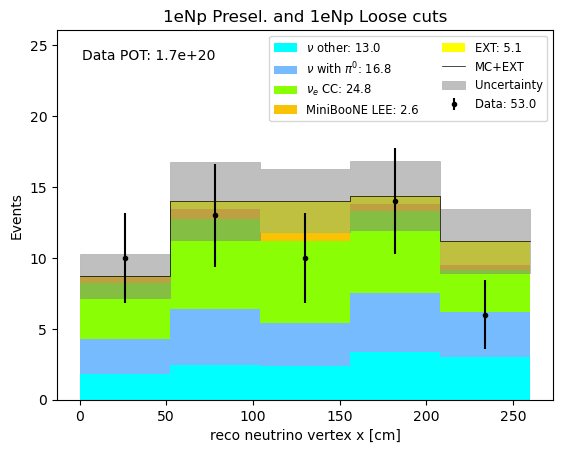
\includegraphics[width=\linewidth]{technote/SystematicsSensitivity/Figures/Run1_Vertex_X_Alex.png}
        \caption{Run 1, pre-fix.}
    \end{subfigure}%
    \begin{subfigure}{0.5\linewidth}
        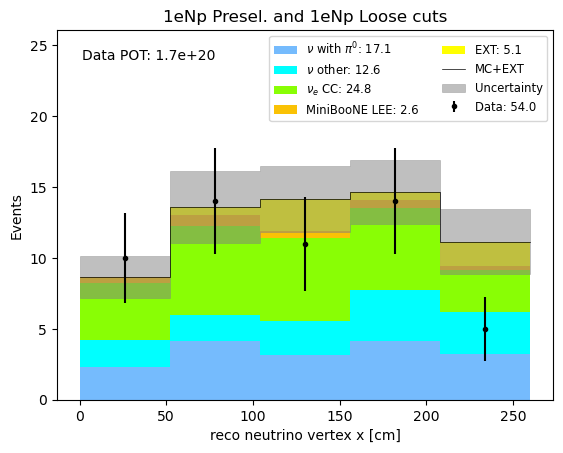
\includegraphics[width=\linewidth]{technote/SystematicsSensitivity/Figures/Run1_Vertex_X_Alex_BugFix.png}
        \caption{Run 1, post-fix.}
    \end{subfigure}
    \begin{subfigure}{0.5\linewidth}
        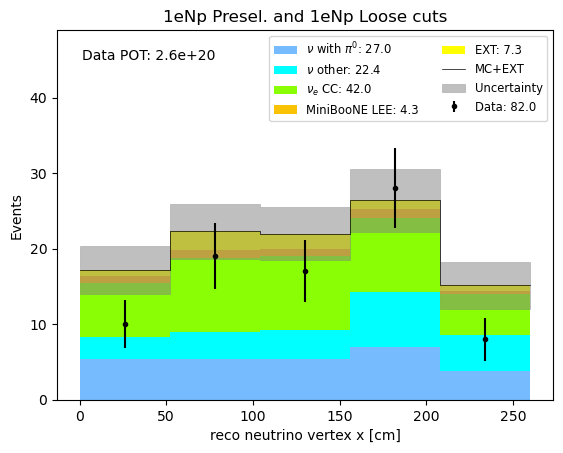
\includegraphics[width=\linewidth]{technote/SystematicsSensitivity/Figures/Run2_Vertex_X_Alex.png}
        \caption{Run 2, pre-fix.}
    \end{subfigure}%
    \begin{subfigure}{0.5\linewidth}
        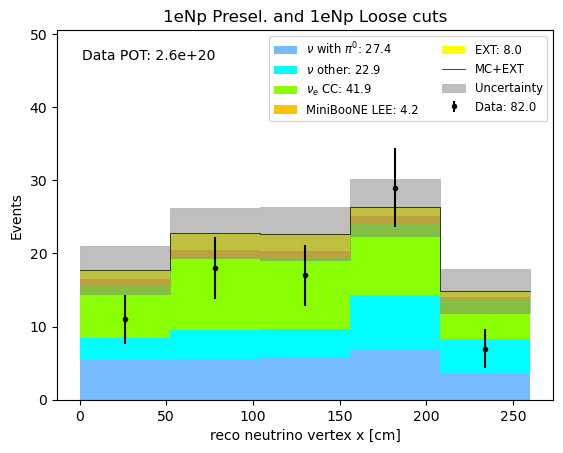
\includegraphics[width=\linewidth]{technote/SystematicsSensitivity/Figures/Run2_Vertex_X_Alex_BugFix.png}
        \caption{Run 2, post-fix.}
    \end{subfigure}
    \begin{subfigure}{0.5\linewidth}
        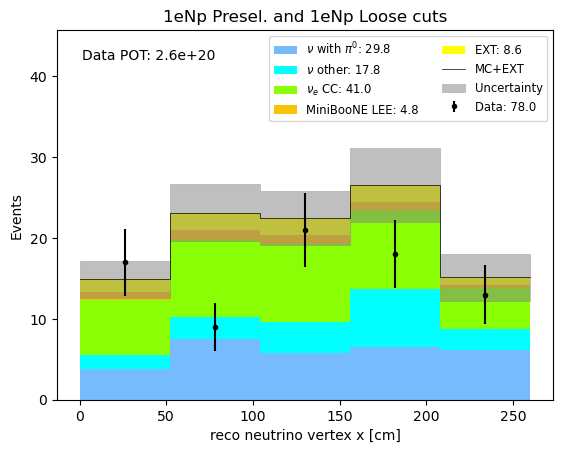
\includegraphics[width=\linewidth]{technote/SystematicsSensitivity/Figures/Run3_Vertex_X_Alex.png}
        \caption{Run 3, pre-fix.}
    \end{subfigure}%
    \begin{subfigure}{0.5\linewidth}
        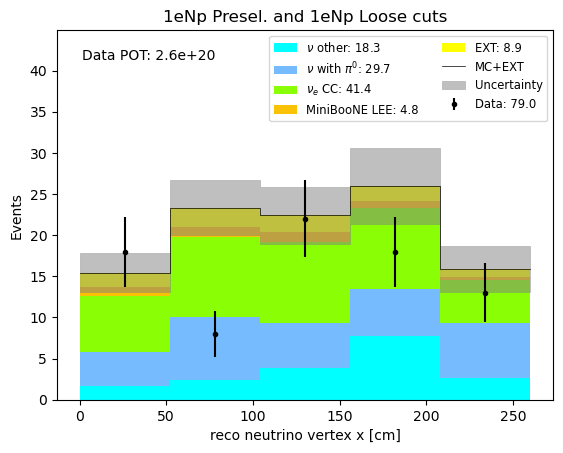
\includegraphics[width=\linewidth]{technote/SystematicsSensitivity/Figures/Run3_Vertex_X_Alex_BugFix.png}
        \caption{Run 3, post-fix.}
    \end{subfigure}
    \caption{Comparison of and data and MC predictions using ntuples generated before and after the FSI reweighting bug-fix was introduced introduced. The data and MC predictions are consistent within the expected level of variation from processing inefficiencies.}
    \label{fig:FSIBugFixValidation}
\end{figure}

\subsubsection{EXT smoothing} (Alex, in progress)
\label{sec:ext_smoothing}
At the final level of the event selection, the number of EXT events is much too small to reliably produce a non-zero bin count in the analysis histograms. In the previous round of the analysis, an error of 1.4 events was assigned to any bin without any EXT events. This number was derived as the expected error given a uniform prior distribution between 0 and 1 on the expectation value. However, this error assignment could lead to an overly conservative error estimate. For this round, we instead use a KDE to produce a smoothed histogram and calculate the covariance matrix of the smoothed histogram using a bootstrapping technique.

The procedure to produce a smoothed histogram is as follows:
\begin{enumerate}
    \item Fit a gaussian KDE to the data. The bandwidth is automatically chosen using the Silverman's rule. 
    \item For every bin in the histogram, numerically integrate the KDE over the bin range and multiply by the sum of all weights in the sample to produce the expected number of events in that bin. This results in the central value of the histogram.
    \item Repeat steps 1 and 2 100 times using bootstrap samples of the data, but use the same bandwidth as was used to compute the central value. The bootstrap samples are generated by multiplying the weight of every event with a random number drawn from a Poisson distribution with an expectation value of one.
    \item Calculate the covariance matrix of the 100 histograms produced in step 3. This is the covariance matrix of the smoothed histogram.
\end{enumerate}
One issue with this procedure is that the KDE may produce unexpected results when a variable is bounded. For example, the distribution of the cosine of an angle is bounded between -1 and 1 and may be peaked close to one in the case of forward scattering. The KDE would over-smooth this distribution and underestimate the total number of events in the histogram, because it assigns a non-zero probability to values larger than one, which is unphysical. To solve this problem, we use a transformed KDE (TKDE) with a transformation that maps the observed data to the real numbers. For two-sided bounded variables, we use the logit transformation, which is given by $y  = \log\left(\frac{x}{1-x}\right)$, which is applied after first scaling the samples such that the bounds are at 0 and 1. For one-sided bounded variables, first shift (and flip in the case of an upper bound) the data such that the bound is at zero and use the log transformation, $y =  \log(x)$. The Gaussian KDE is then fit to the transformed data, $y$. The probability density is then estimated in the original bounded space using the change of variables formula, $p(x) = p(y)\left|\frac{dy}{dx}\right|$. The covariance matrix is then calculated using the same procedure as above. We demonstrate the effect of the TKDE on the EXT histogram in Fig.~\ref{fig:EXT_smoothing}. The left plot shows the 1D distribution of the cosine of the angle between the track and shower, where the bounded KDE smoothing has been applied to the EXT histogram. The right plot shows the unsmoothed EXT histogram and the two KDE smoothed histograms, one using the bounded KDE and one using the standard KDE. The unbounded KDE misses the peak of the distribution close to one, while the bounded KDE gives a more reasonable estimate.
\begin{figure}
    \centering
    \includegraphics[width=0.45\textwidth]{technote/SystematicsSensitivity/Figures/tksh_angle_NPL_NP_smoothed.pdf}
    \includegraphics[width=0.45\textwidth]{technote/SystematicsSensitivity/Figures/tksh_angle_NPL_NP_kde_comparison}
    \caption{Comparison of EXT smoothing methods. Left: 1D distribution of the cosine of the angle between the track and shower, where the bounded KDE smoothing has been applied to the EXT histogram. Right: unsmoothed EXT histogram and the two KDE smoothed histograms, one using the bounded KDE and one using the standard KDE.}
    \label{fig:EXT_smoothing}
\end{figure}
Which boundary treatment to use for each variable is decided automatically unless explicitly overridden by the user by the following procedure:
\begin{itemize}
    \item If there are fewer than 5 samples, use the standard KDE.
    \item If all samples fall within the bounds of the binning of the variable, the two-sided bounded KDE is used.
    \item If there are samples above the upper bound and below the lower bound, the standard KDE is used.
    \item If any samples fall above (below) the upper (lower) bound, the one-sided bounded KDE is used.
\end{itemize}
Other special cases to consider are those where only one or no sample at all. In the case of only one sample, we use the standard KDE and set the kernel bandwidth equal to the bin width. If there are no samples at all, we treat the histogram as being empty and the errors to zero\todo{Should we set non-zero errors in this case?}.

\subsubsection{DetVar systematics}
\todo{Are we assuming Run123 detvars for Run 1-5? Probably true for first sensitivites.} 
\todo{Include a table which lists MC stats available on DetVar samples.}
In contrast to the first iteration of the analysis, we include bin-to-bin correlations in our estimate of the detector uncertainties. We use the same detector variations as were used in the first round of the analysis an treat each variation as a $1\sigma$ unisim variation. We produce histograms of the detector variations using the same event selection and binning that we also apply to the analysis and then calculate the fractional covariance matrix for each variation as 
\begin{equation}
    C_{\text{var}, ij} = (\mu_{\text{var},i} - \mu_{\text{cv},i})(\mu_{\text{var},j} - \mu_{\text{cv},j})/(\mu_{\text{cv},i}\mu_{\text{cv},j})\;,
\end{equation}
where $\mu_{\text{var},i}$ and $\mu_{\text{cv},i}$ are the expectation values in the variation histogram and the central value, respectively. The total covariance of the detector uncertainties is the sum of the covariances of all variations. Histograms of the detector variations are shown in \cref{fig:unisim-covariance}.
\begin{figure}
    \begin{subfigure}{0.45\textwidth}
        \missingfigure{Histograms of unisim variations}
    \end{subfigure}
    \begin{subfigure}{0.45\textwidth}
        \missingfigure{Detector fractional covariance}
    \end{subfigure}
    \caption{Histograms of the unisim variations (left) and total fractional covariance matrix (right) in the XXX selection.}
    \label{fig:unisim-covariance}
\end{figure}
\subsubsection{Signal model systematics}

\subsection{systematics summary}

The total systematics error budget is shown in the table of Fig.~\ref{fig:systematicsbudget}.

\begin{center}
\begin{figure}[h]
    \includegraphics[width=1.00\textwidth]{technote/SystematicsSensitivity/Figures/systematicsbudget.png}
    \caption{Enu spectrum before/after constraint.}
    \label{fig:systematicsbudget}
\end{figure}
\end{center}

\newpage
\subsection{Constraints}

%\todo[inline]{Do these include the full dataset (minus run 4a), with the updated run 3 sample?}

Describe briefly, refer to older analysis.

The spectra before and after the application of the sideband constraint are shown in \cref{fig:constraint}. The constraint was calculated using the inclusive $\nu_\mu$ selection shown in \cref{fig:sideband-numu-crt}. The correlation between all bins of the included spectra is shown in \cref{fig:correlation-genie}, which includes the correlations due to GENIE, flux and reinteraction multisim universes and GENIE unisim knobs.

\begin{center}
\begin{figure}[h]
    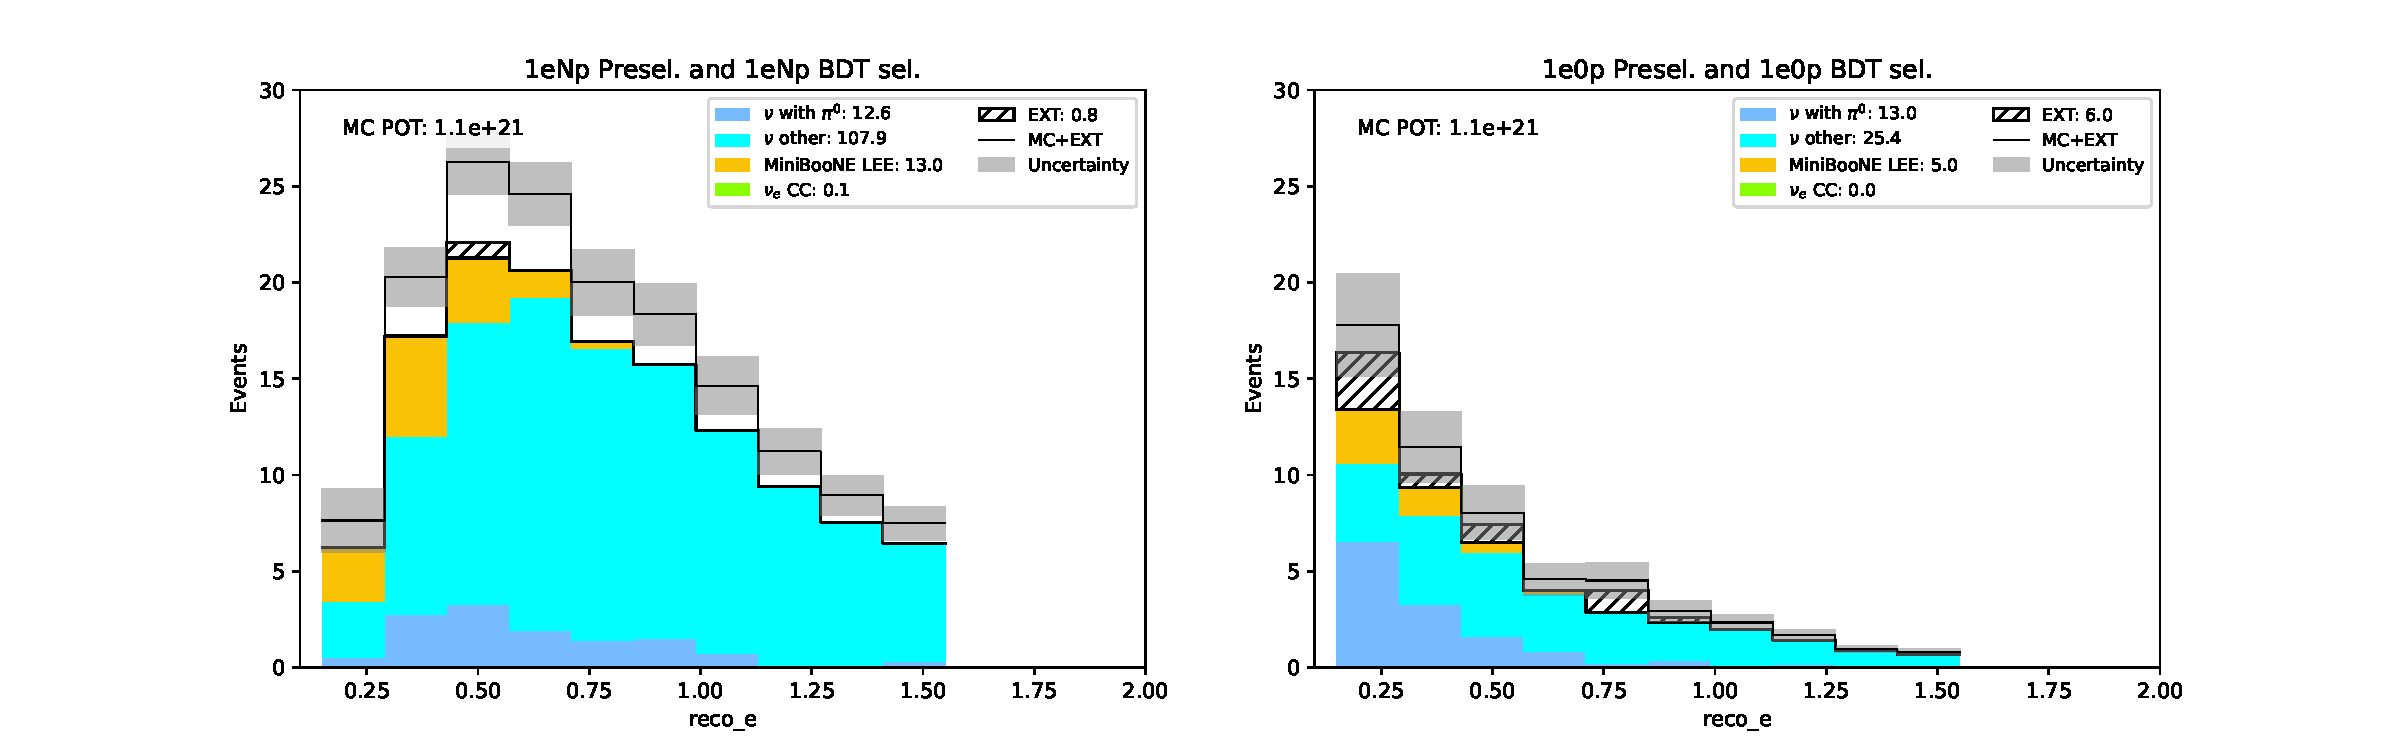
\includegraphics[width=1.00\textwidth]{technote/SystematicsSensitivity/Figures/signals_runs_1-5_constrained.pdf}
    \caption{Signal spectra including sideband constraint correction. The stacked histograms were calculated without constraint corrections,  while the solid black line labeled "MC + EXT" is adjusted to account for the measured sideband data.}
    \label{fig:constraint}
\end{figure}
\end{center}

\begin{figure}
    \centering
    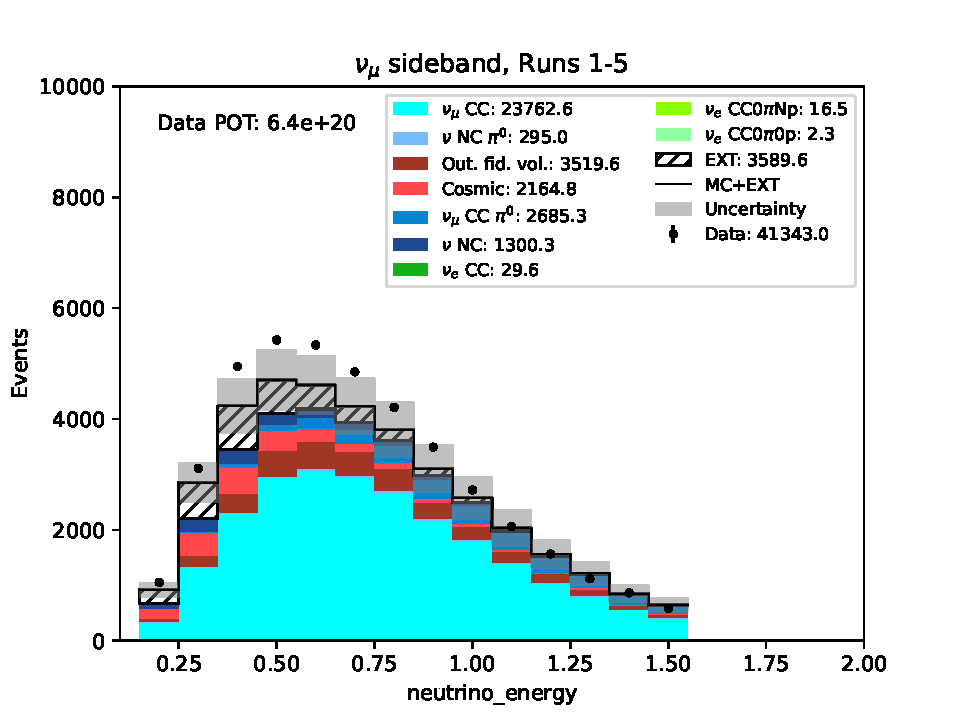
\includegraphics[width=0.7\linewidth]{technote/SystematicsSensitivity/Figures/sideband_numu_runs_1-5.pdf}
    \caption{Inclusive $\nu_\mu$ selection with CRT cuts used to compute the constraints in \cref{fig:constraint}.}
    \label{fig:sideband-numu-crt}
\end{figure}

\begin{figure}
    \centering
    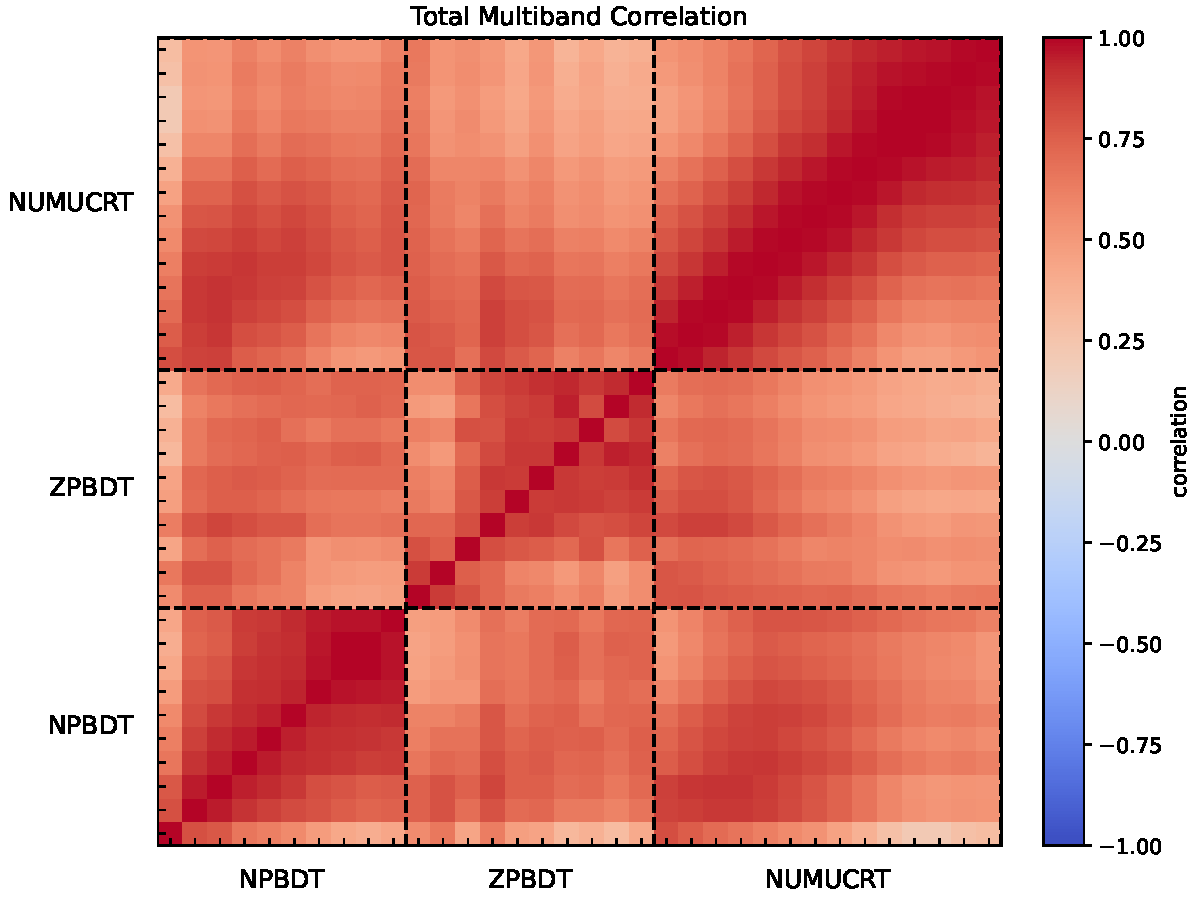
\includegraphics[width=0.7\linewidth]{technote/SystematicsSensitivity/Figures/multiband_correlation_runs_1-5_total.pdf}
    \caption{Total correlation between signal bands and the inclusive $\nu_\mu$ sideband.}
    \label{fig:correlation-genie}
\end{figure}

Show quantitative predicted events and uncertainty (including reduction in uncertainty) before/after constraint. See Table of Fig.~\ref{fig:constrainttable}.

\begin{center}
\begin{figure}
    \includegraphics[width=1.00\textwidth]{technote/SystematicsSensitivity/Figures/constrainttable.png}
    \caption{Impact of constraint.}
    \label{fig:constraint} 
\end{figure}
\end{center}

\subsubsection{Updates to Constraint Procedure (Giuseppe, work in progress)}
\label{sec:construpd}

In the first round of the analysis we used a $\nu_\mu$ inclusive selection to constrain the $\nu_e$ prediction in the signal region. The strategy behind this choice was to leverage a robust procedure that would maximally constrain the flux. With a larger data set available for the second round of MicroBooNE LEE analyses, a more advanced constraint procedure can be defined. The idea of a multi-channel constraint has already been used by the inclusive analysis in the first round of LEE results. The pionless analysis includes two signal channels, with and without visible protons. A substantial background from NC $\pi^0$ events is present in the low energy region of the 0p selection. Therefore, we developed new selections with the goals of:
\begin{itemize}
    \item constraining separately the channels with and without visible protons (with a selection that matches the hadronic topology of the $\nu_e$ selection);
    \item constraining the dominant NC $\pi^0$ background in $1\mathrm{e}0\mathrm{p}0\pi.$
\end{itemize} 

As we did in the first round of the analysis we restrict the constraint selections to run periods with reliable CRT information for cosmic background rejection. In this analysis, this means using run3 (after run 14114), 4 (excluding 4a), and 5.

The first step is to update the inclusive $1\mu$ selection to a $1\mu0\pi$ selection. We do this by requiring that there is only one track identified as a muon (which suppresses the charged pion contribution) and vetoing the presence of showers in the event (to suppress neutral pions). We also tested a configuration allowing at most 1 shower. In Fig.~\ref{fig:npinumusel} (left) we show the number of pions in the events selected with the $1\mu$ (old) and $1\mu0\pi$ (new) selection: the fraction of events with no pions increases from 65\% to 80\%. Then we can separate the events passing the $1\mu0\pi$ selection based on the presence or absence of tracks identified as proton candidates. In the 0p case we observe a significant contamination from cosmic background, so for this selection we tighten the Pandora topological score cut to 0.2 (Fig.~\ref{fig:npinumusel}, right. The resulting $1\mu0\mathrm{p}0\pi$ and $1\mu0\mathrm{p}0\pi$ selections are shown in Fig.~\ref{fig:numu0pisels}.

\begin{center}
\begin{figure}
    \centering
    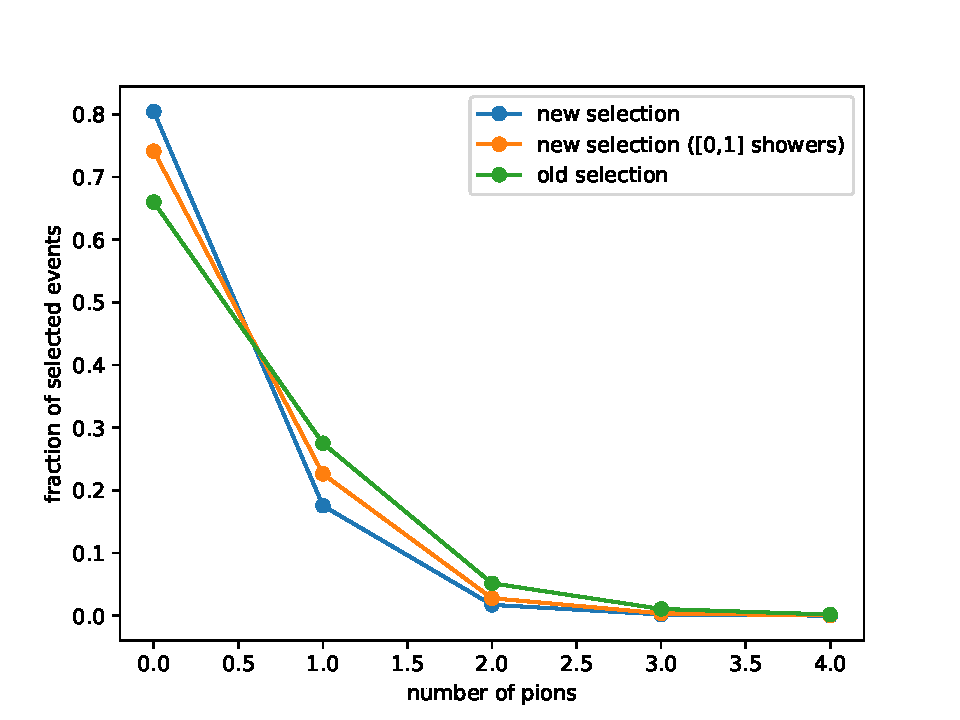
\includegraphics[width=0.45\textwidth]{technote/SystematicsSensitivity/Figures/npi_musel.pdf}
    \hfill
    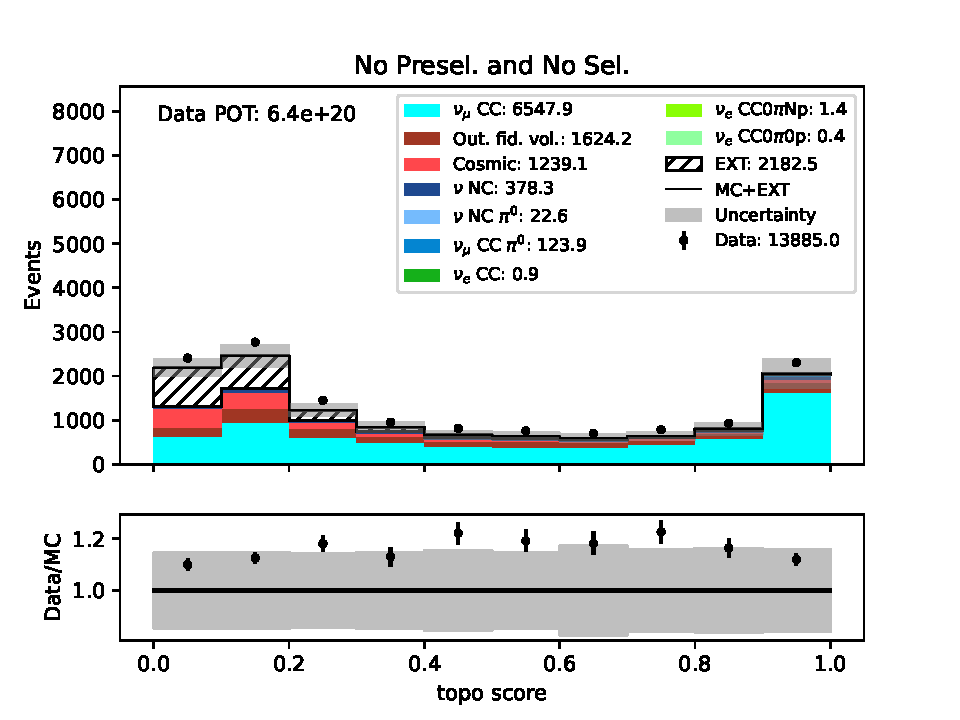
\includegraphics[width=0.45\textwidth]{technote/SystematicsSensitivity/Figures/topological_score_1mu0p0pi.pdf}
    \caption{Left: number of true pions in events passing the $\nu_\mu$ selections described in the text. Right: topological score for the $\nu_\mu$ selection after requiring no showers and only one track identified as a muon. In order to define the $1\mu0\mathrm{p}0\pi$ selection, a cut is placed at 0.2.}
    \label{fig:npinumusel} 
\end{figure}
\end{center}

\begin{figure}
    \centering
    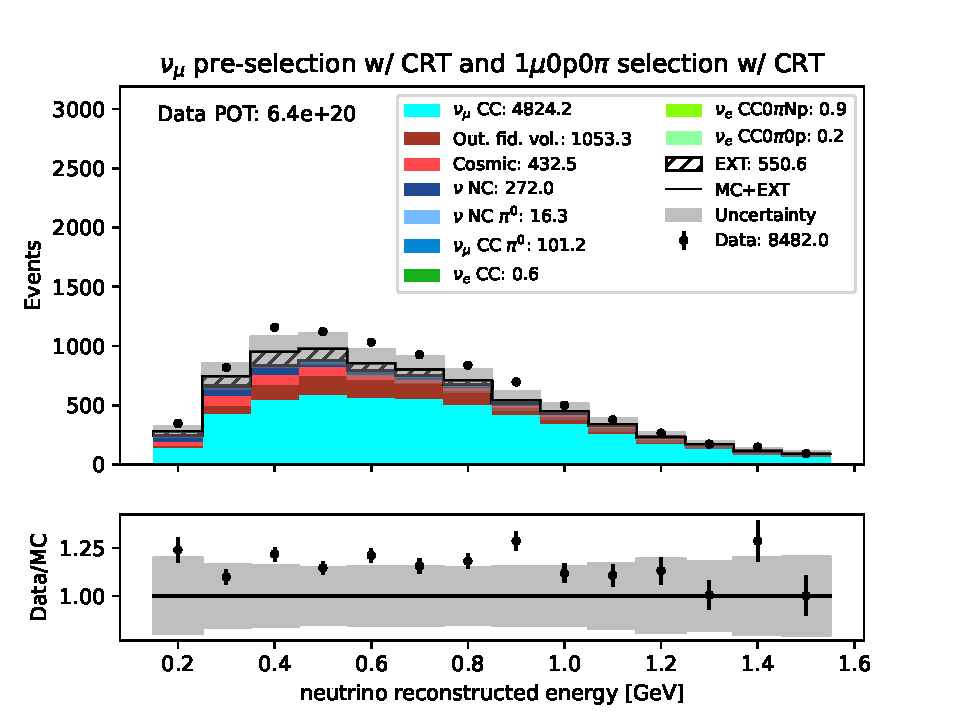
\includegraphics[width=0.45\textwidth]{technote/SystematicsSensitivity/Figures/reco_e_1mu0p0pi.pdf}
    \hfill
    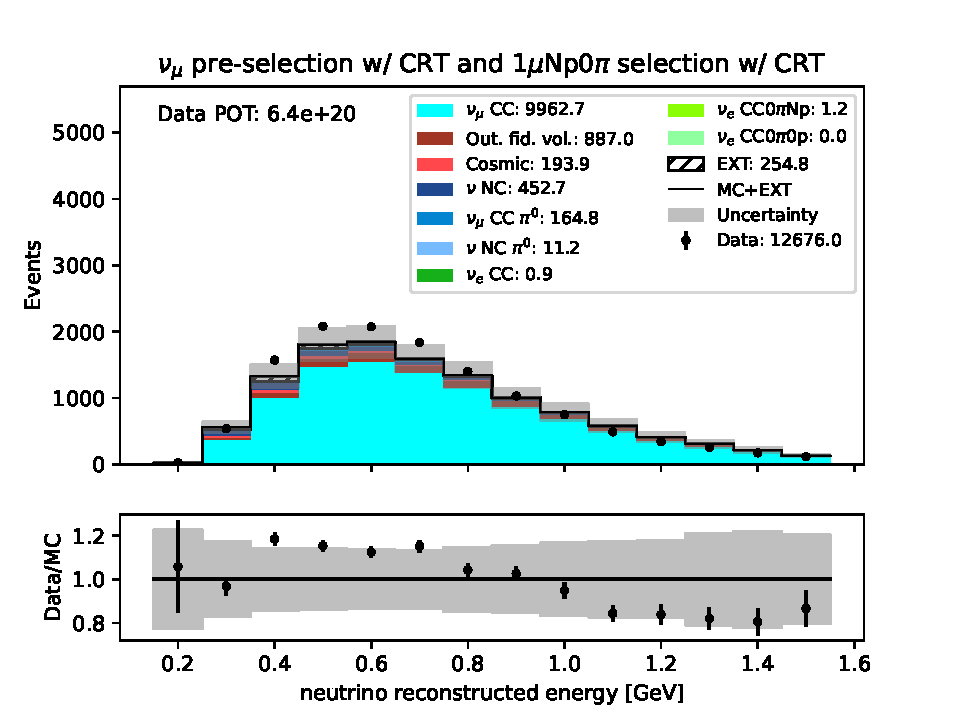
\includegraphics[width=0.45\textwidth]{technote/SystematicsSensitivity/Figures/reco_e_1muNp0pi.pdf}
    \caption{Updated $\nu_\mu$ selections for the constraint: $1\mu0\mathrm{p}0\pi$ (left) and $1\mu\mathrm{Np}0\pi$ (right).}
    \label{fig:numu0pisels}
\end{figure}

We then define a selection to constrain the NC$\pi^0$ background in the $1e0\mathrm{p}0\pi$ selection. For this purpose we leverage the 2-shower sideband, and apply the $1e0\mathrm{p}0\pi$ selections after requiring two showers instead of one (Fig.~\ref{fig:2shr0p}). A high statistics option with use the "loose" selection with the CRT cuts. This selection achieves a good NC$\pi^0$ purity (65\%). Another option that may maximise the phase space overlap with the NC$\pi^0$ events passing the $\nu_e$ selection is to apply the BDT selection. In this case the tighter selection is enough to suppress the cosmic background, so we do not need to use the CRT cuts and we can leverage the full data set.

\begin{figure}
    \centering
    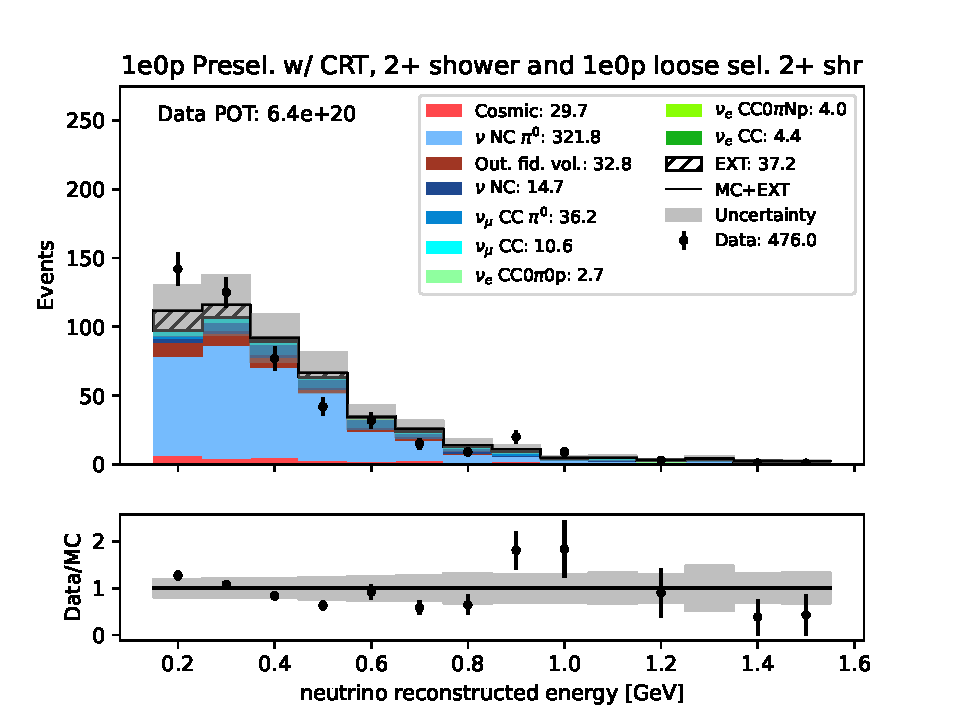
\includegraphics[width=0.45\textwidth]{technote/SystematicsSensitivity/Figures/reco_e_2shr_loose_1e0p0pi.pdf}
    \hfill
    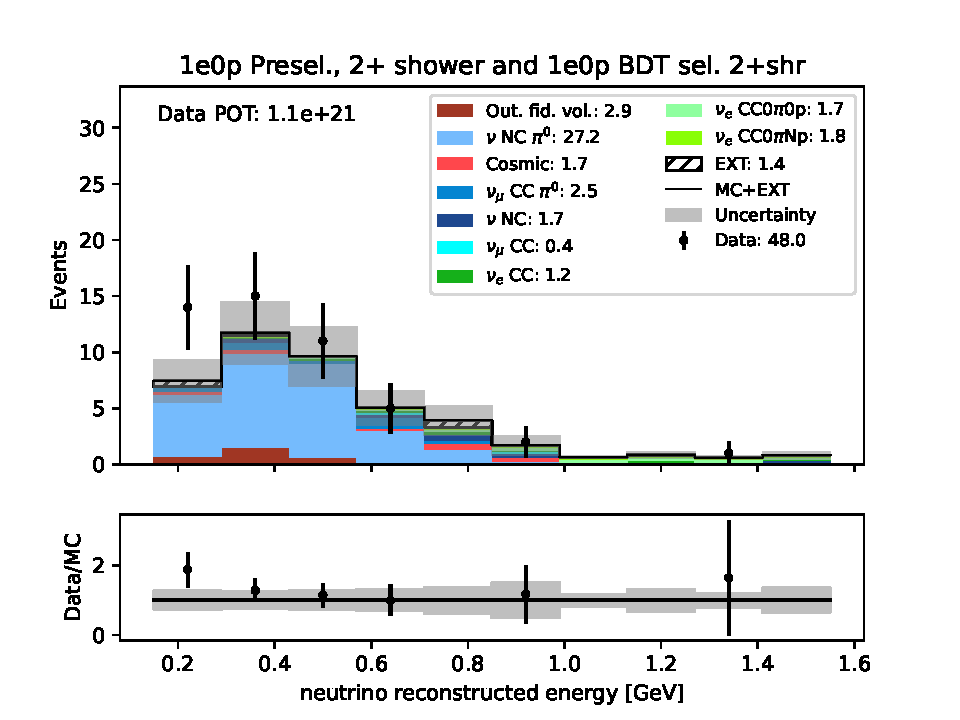
\includegraphics[width=0.45\textwidth]{technote/SystematicsSensitivity/Figures/reco_e_2shr_bdt_1e0p0pi.pdf}
    \caption{NC$\pi^0 0\mathrm{p}$ constraint selection. Left: loose selection with CRT. Right: BDT selection without CRT over the full data.}
    \label{fig:2shr0p}
\end{figure}

While they are being finalized, we plan to use these selections in this round of analysis. So events in the $\nu_e$ selections will be simultaneously constrained from the 3 channels defined above. We may also explore constraining based on other kinematic variables (muon momentum and angle for the muon selections, leading shower momentum and angle for NC $\pi^0$).

TO DO: when we look at the covariance matrix (or better the correlation matrix), do we see as expected larger correlations between Np-Np channels, and between 0p-0p and 0p-NC?\todo{Intepretation}
\begin{figure}
    \centering
    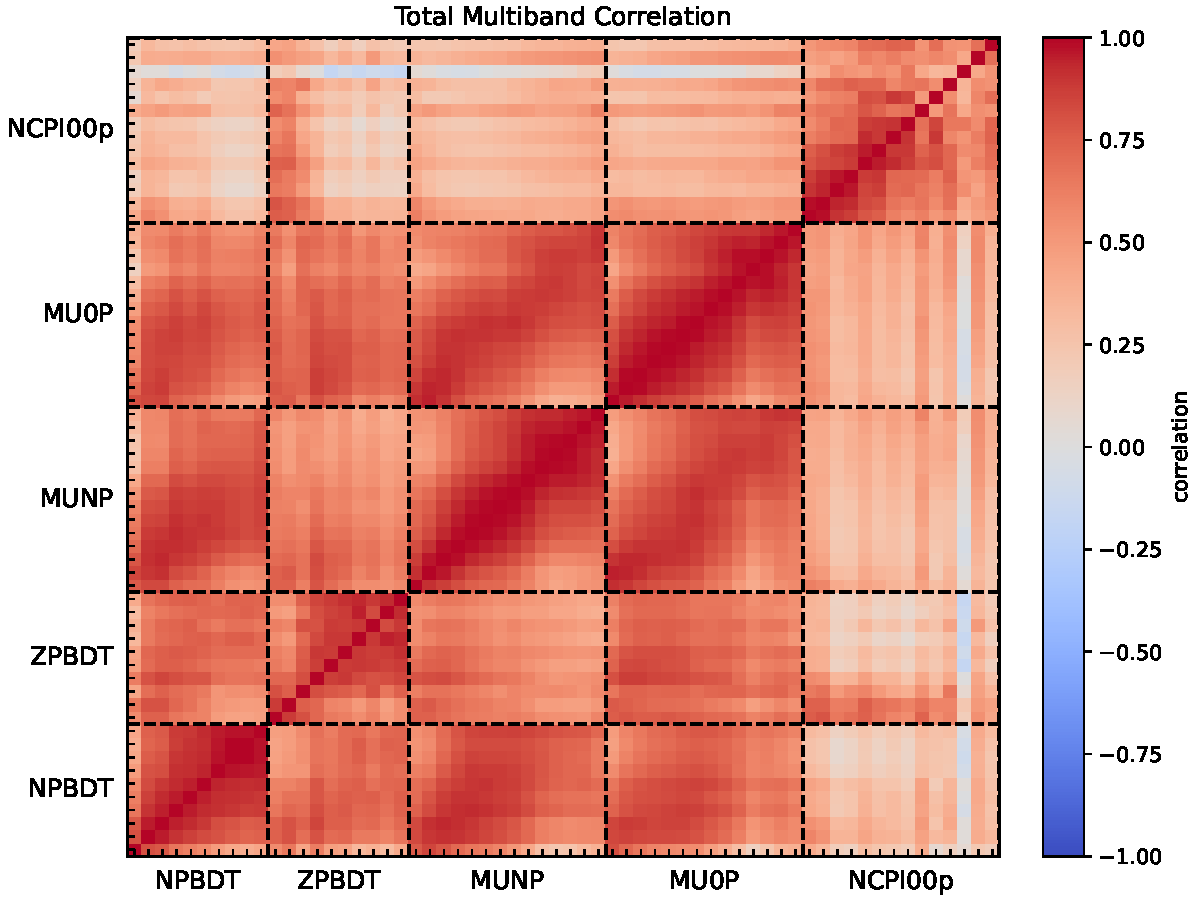
\includegraphics[width=0.95\linewidth]{technote/SystematicsSensitivity/Figures/newconstraintscorrelations.pdf}
    \caption{Total correlation between the $1\mathrm{e}N\mathrm{p}0\pi$, $1\mathrm{e}0\mathrm{p}0\pi$, $1\mu\mathrm{Np}0\pi$ and the NC$\pi^0 0\mathrm{p}$ constraint selections.}
    \label{fig:sidebands-total-correlation}
\end{figure}

\newpage
\subsection{Sensitivity}
\label{sec:sensitivity}

\subsubsection{Simple Hypothesis Test}

Distribution of test statistic for background-only and signal models, with extracted median sensitivity. See. Fig.~\ref{fig:simplehypothesis}.

\begin{figure}[h]
    \centering
    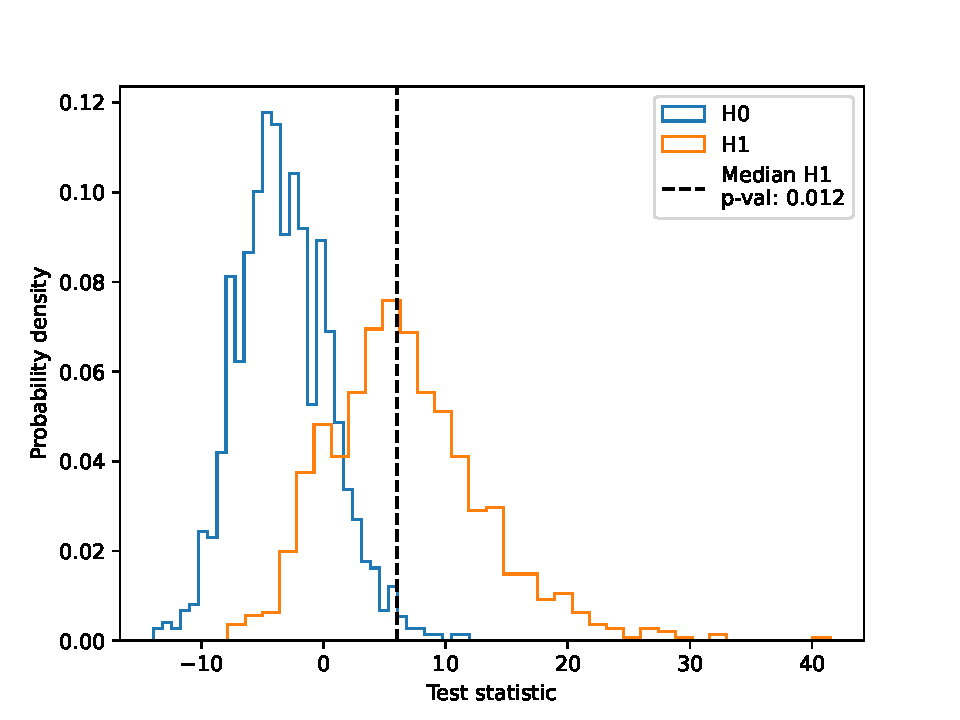
\includegraphics[width=0.7\textwidth]{technote/SystematicsSensitivity/Figures/two_hypothesis_test_runs_1-5_with_crt.pdf}
    \caption{Median sensitivity of the simple two-hypothesis test including runs 1-5, with the inclusive $\nu\mu$ sideband selection used as constraint.}
    \label{fig:simplehypothesis} 
\end{figure}

Fig.~\ref{fig:simplehypothesisresults} shows the expected sensitivity for the simple hypothesis test.

\begin{center}
\begin{figure}[h]
    \includegraphics[width=1.00\textwidth]{technote/SystematicsSensitivity/Figures/simplehypothesisresults.png}
    \caption{Impact of constraint.}
    \label{fig:simplehypothesisresults} 
\end{figure}
\end{center}

\newpage
\subsubsection{Signal strength fit}

The signal strength sensitivity results are shown in Fig.~\ref{fig:signalstrengthsensitivity}.
\begin{center}
\begin{figure}[h]
    \includegraphics[width=1.00\textwidth]{technote/SystematicsSensitivity/Figures/signalstrengthsensitivity.png}
    \caption{Impact of constraint.}
    \label{fig:signalstrengthsensitivity} 
\end{figure}
\end{center}

%\newpage
%\subsubsection{Validation of sensitivity vs. SBNFit benchmark}
